% !TEX root = _yoko.tex

% ==========================================
% プロジェクト予稿（1P）の本文
% ==========================================

\section{はじめに}
近年，音楽や映画といった時系列メディアを対象とした多様な作品分析手法が提案されている．これらの分析において，対象作品の視聴や分析方法の検討など，さまざまな要素が含まれるが，場面分けは多くの分析手法に共通する作業である．分析の手法として自動で行う手法と手動で行う手法が存在する．自動分割の課題として場面分けが細かすぎたり，複数の解釈の視点が存在したりする．そこで，場面分けをする際人の介入が必要となる．

そこで本研究では，人の解釈の介入が存在する手動で場面分けされていたものはどういった手法が存在するのか文献調査を行う．そして，そこから抽出された場面分けの切り方を参考に，1つの作品を対象として比較分析を行い，考察を行っていく．
\section{研究背景}
時系列メディアを扱った分析はさまざまな手法で行われている．分析をする上で様々な作業があるが，対象作品の場面分けは多くの分析手法に共通するものである．場面分けの手法として，自動で分割する方法や手動で分割する方法が存在する．

自動で分割するシステムの課題として，場面分けが1秒や2秒になってしまい，一つ一つの場面が細かくなってしまうことが問題となる．また，分析を行う際，複数の解釈が存在するため場面のグルーピングの方針を検討する必要がある．

そこで，場面分けをする際人の解釈の介入が必要となる．つまり，自動分割した場面分けにさらに手動で分割やグルーピングをする必要がある．

本研究では，手動で分析する際，どのような基準をもって場面分けを行っているか調査を行う．調査方法として，CiNii\cite{CiNii}を利用し，手動によるメディア分析を対象とした論文を抽出・調査した．分析対象は以下の8つのカテゴリに絞った：演劇，小説，プレゼンテーション，映画，将棋，映像，作品分析，感情分析．これらの論文から，さらに「分析」と「場面分け」に関する記載があるものを抽出し，対象を絞り込んだ．
次に，抽出された論文に記載された場面分けに着目し，各分析者がどのような観点や理論に基づいて作品の場面分けを行っているのかを調査を行った．その結果，該当する論文は合計84件が抽出された．そのうち，「分析」と「場面分け」に関する記載が明確に認められる論文は12件に絞られた．
\subsection{調査に対する結果}
文献調査によって選定された論文の場面の切り方とグルーピング方法をまとめた．切り方の中でも，物語内の事象と伏線となる場面に注目をした．注目した2種類の切り方を使って1つの作品の事象をどのようして場面分けを行うのか分析を行う．

\section{同一作品の解釈}
\subsection{比較分析}
分析手法として，被験者に対象作品の始まりから終わりまでを場面分けを行ってもらい，Googleのスプレットシートに記載してもらう．被験者は3人とし，属性は18歳から20歳男女学生である．

場面分けをする条件として文献調査で注目した2種類の切り方を元にして，場面転換が起こった時，登場人物が変わった時，話の伏線と回収になる場面が起こった時に設定した．被験者は条件を提示され場面分けを行ったとき，映像のどの場面で設定した場面分けをすると解釈するかは被験者によって異なっていくのではないかと考えた(図1)．
figref{fig:hikaku}
\begin{figure}[tb]
\centering
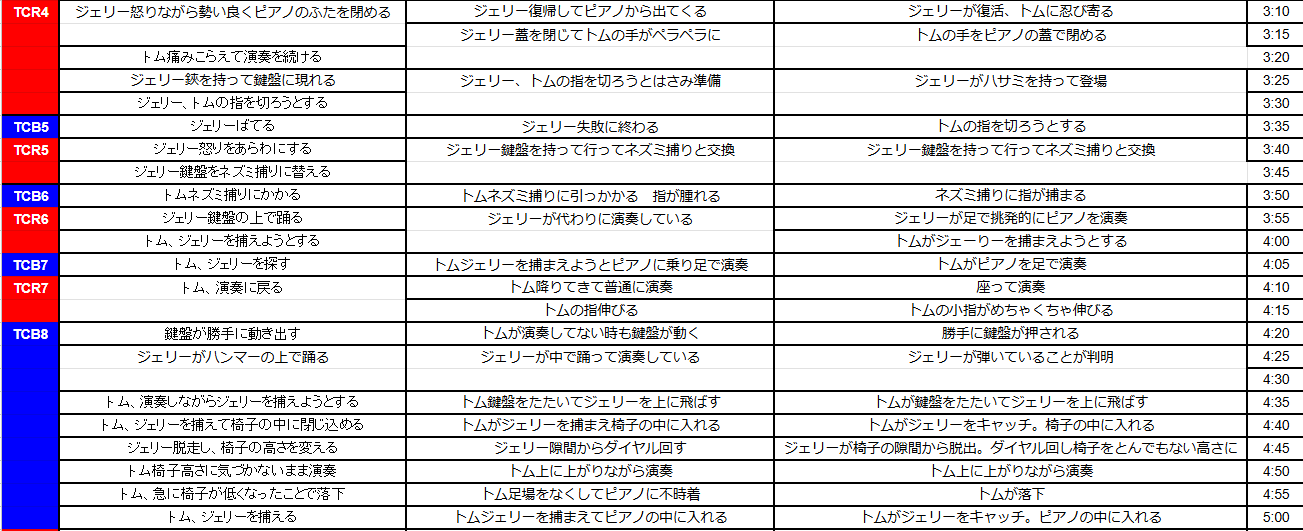
\includegraphics[width=\hsize]{fig/fig1-hikaku.png}
\caption{比較分析例}
\label{fig:hikaku}
\end{figure}
\subsection{対象作品}
1940年から1958年までに公開された短編アニメーションシリーズのトムとジェリー\cite{tom}から4作品を対象とする．トムとジェリーを対象とした理由としては，登場人物が少なく，一話完結で，短編かつ話が数多く存在したためである．対象とする話としては，The Two Mouseketeers・The Cat Concerto・The Missing Mouse・Mouse Troubleの4作品である．

\subsection{場面分けが異なる要因}
調査と分析によって得られた場面分けが異なる要因として，物語内の場面の転換，鑑賞者の物語内における視点，行動の細分化，登場人物の感情や行動や関係性，鑑賞者の感情なのではないかと考えた．

\section{まとめ}
本研究では，場面分けにたいして調査，比較分析，考察，提案を行ってきた．

調査として作品分析を行っている論文を収集し，場面分けの現状を調べた．

そのことを踏まえて短編アニメーション作品のトムとジェリーを対象として被験者に場面分けを行ってもらい比較，考察を行った．
その考察を踏まえて場面分けが異なる要因として場面転換，鑑賞者の物型に対する視点，行動の細分化，登場人物の感情や行動や関係性，鑑賞者の感情ではないかと提案した．
